\chapter{אנטומיה של יום דיגיטלי}

\begin{epigraph}{}
אנחנו לא מבזבזים זמן על המסך. אנחנו משלמים בו. השאלה היא רק מה אנחנו מקבלים בתמורה.
\end{epigraph}

\section{6 שעות ו-40 דקות}

לאיכר בימי הביניים היה יום ברור. הוא קם עם השמש, עבד בשדה, אכל, התפלל וישן כשהחשיך. השמש הייתה השעון, העונות היו לוח השנה, והכנסייה הייתה ערוץ החדשות היחיד.

היום שלנו בנוי אחרת. הוא מחולק לא לפי השמש אלא לפי המסכים. לפי הדוח הגלובלי \en{Digital 2024}, משתמש אינטרנט טיפוסי מבלה ברשת כ-6 שעות ו-40 דקות ביום, כ-400 דקות \parencite{kemp2024}. שנה קודם לכן היה המספר 6 שעות ו-36 דקות. כלומר, אחרי שנים של זינוק, הוא כמעט התייצב. אולי הגענו לתקרה. אולי פשוט נגמרו לנו השעות.

כדי להבין את המספר הזה, כדאי לחשוב עליו כעל תקציב. אם אתם ישנים כשמונה שעות, נשארות לכם כשש-עשרה שעות שבהן אתם ערים. מתוכן, כ-\num{40\%} עוברות ברשת. ולא מדובר רק בגלילה בטלפון: גם העבודה מול המחשב, הסדרה בערב והניווט ברכב נכנסים לחשבון. הרשת היא כבר לא מקום שהולכים אליו. היא המקום שבו אנחנו נמצאים.

\section{לאן הולך הזמן}

טבלה~\ref{tab:daily-time} מפרקת את התקציב היומי לכמה מרכיבים מרכזיים, לפי הנתונים שפורסמו בדוח.

\begin{table}[htbp]
\centering
\caption{זמן יומי ממוצע לפי פעילות (משתמש טיפוסי, 2024)}
\label{tab:daily-time}
\begin{tabularx}{0.9\textwidth}{@{}X c@{}}
\toprule
\textbf{פעילות} & \textbf{זמן ליום (שעות:דקות)} \\
\midrule
סך כל הזמן ברשת & \num{6:40} \\
רשתות חברתיות & \num{2:23} \\
טלוויזיה משודרת (ליניארית) & \num{1:44} \\
טלוויזיה בכל הפורמטים, כולל סטרימינג & \num{>3:00}\textsuperscript{*} \\
\bottomrule
\end{tabularx}

\vspace{0.3em}
{\small\sffamily מקור: \textcite{kemp2024}. הפעילויות חופפות זו לזו, ולכן אינן מסתכמות לסך הכולל. \textsuperscript{*}הדוח מוסר רק שהזמן עולה על שלוש שעות, בלי ערך מדויק.}
\end{table}

הרשתות החברתיות לבדן לוקחות כ-2 שעות ו-23 דקות ביום \parencite{kemp2024}. נסו להשוות את זה לזמן שאתם מקדישים לארוחות, לספורט ולשיחה פנים אל פנים עם בני המשפחה, ביחד. המעניין הוא שהמספר הזה דווקא ירד מעט, מ-2 שעות ו-31 דקות בשנה הקודמת, אבל לפי הדוח עצמו, רוב הירידה נובעת משינוי בשיטת המדידה \parencite{kemp2024}. גם לסטטיסטיקה יש מצבי רוח.

והטלוויזיה? הקופסה שהייתה פעם מרכז הסלון לא מתה. היא רק שינתה צורה. הצפייה בטלוויזיה המשודרת ירדה לשעה ו-44 דקות ביום, לעומת שעה ו-58 דקות ב-2019, אבל כשמחברים את כל הפורמטים, כולל סטרימינג, מגיעים ליותר משלוש שעות ביום \parencite{kemp2024}. הטלוויזיה לא נעלמה. היא נכנסה לטלפון.

\begin{alertbox}[למה הטבלה לא "מסתכמת"]
אפשר לצפות בסדרה תוך כדי גלילה בטלפון, ולשמוע פודקאסט בזמן שעונים להודעות. לכן אסור לחבר את השורות בטבלה ולצפות לקבל את הסך הכולל. אנחנו לא רק מבלים זמן רב מול מסכים. לעיתים קרובות אנחנו מבלים אותו מול כמה מסכים בבת אחת.
\end{alertbox}

\section{מפת העולם של זמן המסך}

ממוצע עולמי מסתיר הבדלים עצומים. איור~\ref{fig:daily-time} משווה בין כמה מדינות. בדרום אפריקה משתמש טיפוסי מבלה ברשת כ-9 שעות ו-24 דקות ביום. בברזיל כ-9 שעות ו-13 דקות, ובפיליפינים כ-8 שעות ו-52 דקות. בקצה השני נמצאות דרום קוריאה, עם כ-5 שעות ו-19 דקות, ודנמרק, עם כ-5 שעות ו-8 דקות \parencite{kemp2024}. ביפן הממוצע נמוך עוד יותר, פחות מארבע שעות ביום \parencite{kemp2024}.

% גרף Python: python/make_graphs.py → images/daily_time.png
\begin{figure}[htbp]
\centering
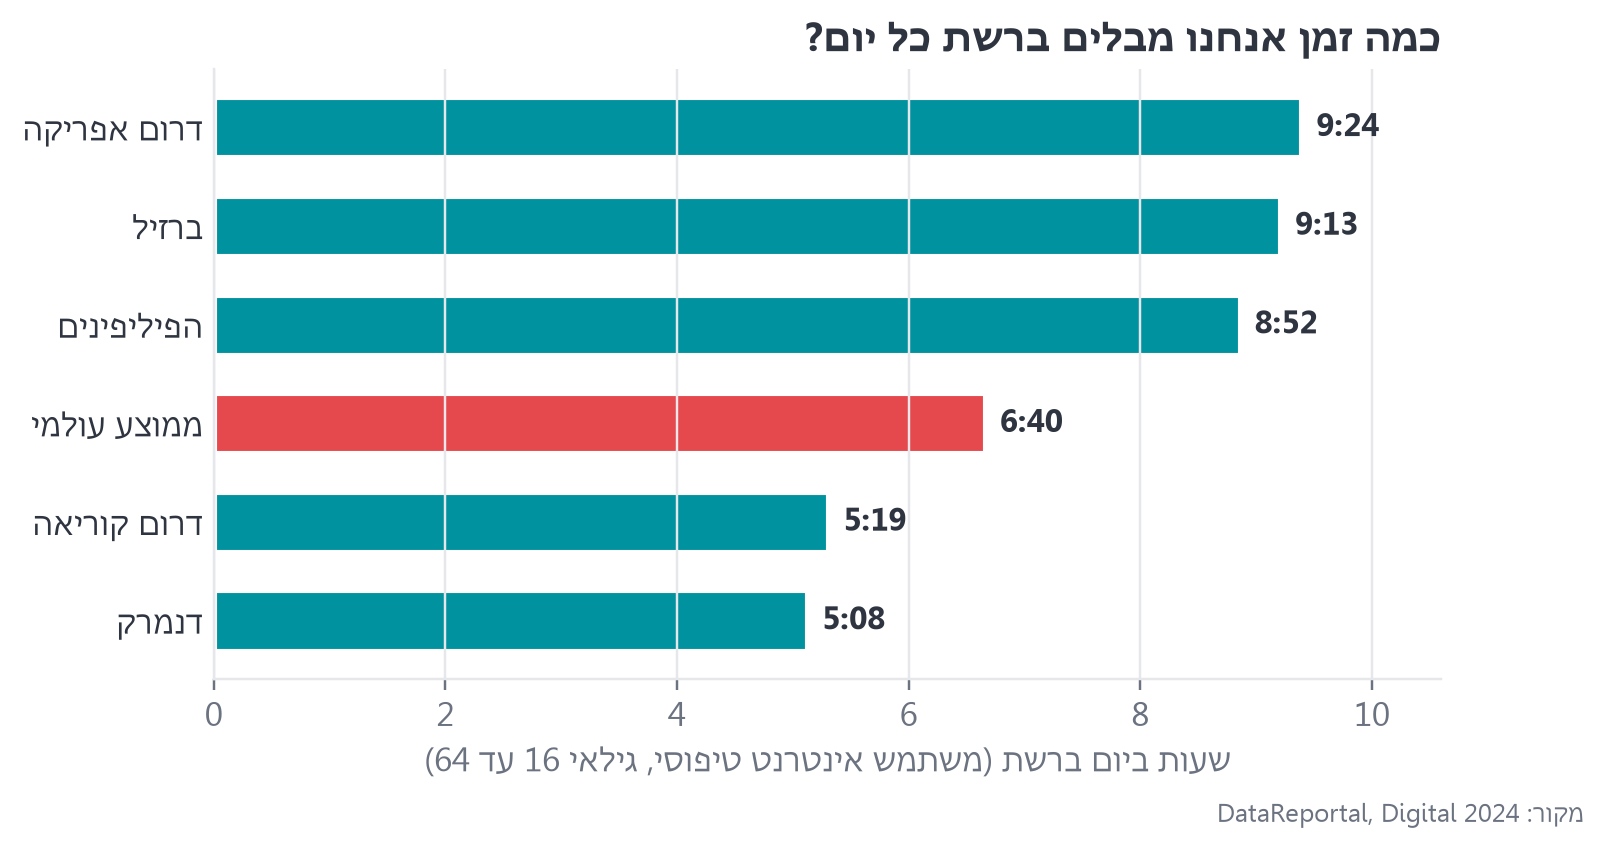
\includegraphics[width=0.92\textwidth]{images/daily_time.png}
\caption[זמן יומי ממוצע ברשת לפי מדינה]{זמן יומי ממוצע ברשת במדינות נבחרות לעומת הממוצע העולמי \parencite{kemp2024}. הגרף נוצר ב-\en{Python}.}
\label{fig:daily-time}
\end{figure}


איך מסבירים את הפער? אפשר היה לנחש שהמדינות העשירות והטכנולוגיות ביותר יובילו. אבל דרום קוריאה, אחת המדינות המחוברות והמתקדמות בעולם, נמצאת דווקא סמוך לתחתית האיור. חשוב לזכור שאת המדינות באיור בחרנו אנחנו, מתוך אלה שהדוח מזכיר בטקסט, כדי להמחיש את הטווח. זו לא רשימה מלאה ולא דירוג. הנתונים לבדם לא מסבירים את הסיבה, וכדאי להיזהר מתשובות מהירות. ייתכן שיש לכך קשר לשעות העבודה, לגיל האוכלוסייה, למזג האוויר או לתרבות של בילוי מחוץ לבית. ייתכן שבמקומות שבהם הטלפון הוא המחשב היחיד, הוא גם הקולנוע, הבנק והכיכר העירונית. הדבר הבטוח היחיד הוא שזמן מסך איננו גזירת גורל טכנולוגית. הוא גם עניין של תרבות.

\begin{factbox}[קנה המידה]
בתחילת \num{2024} היו בעולם כ-\num{5.35} מיליארד משתמשי אינטרנט וכ-\num{5.04} מיליארד "זהויות" ברשתות חברתיות \parencite{kemp2024}. המספר נמוך מ-\num{5.87} המיליארד שבפרק הקודם, כי מדובר במקור אחר: \en{DataReportal} מודד את תחילת השנה ובשיטה משלו, ואילו \en{ITU} מעריך את השנה כולה, ובסדרה המעודכנת. זהויות, לא אנשים: לאדם אחד יכולים להיות כמה חשבונות, ולחשבון אחד יכולים להיות כמה בעלים.
\end{factbox}

\section{הזמן כמטבע}

לכל ציוויליזציה היה מטבע משלה. מלח, צדפים, זהב, שטרות. בעולם הדיגיטלי מתגבש מטבע חדש: \textbf{הזמן שלכם}. כשאפליקציה מציעה לכם שירות "בחינם", היא לא באמת מוותרת על תשלום. היא פשוט גובה אותו בדקות.

הכלכלנים מדברים על "עלות אלטרנטיבית": המחיר האמיתי של כל דבר הוא מה שוויתרנו עליו כדי להשיג אותו. עלות אלטרנטיבית של שעה בגלילה היא שעה של שינה, ספר, ריצה או שיחה. זה לא אומר שהגלילה תמיד גרועה. לפעמים היא בדיוק מה שצריך אחרי יום ארוך. אבל זה אומר שכדאי לפחות לדעת שמשלמים.

וזה מעלה שאלה מטרידה. אם 400 דקות ביום הן תקציב, מי מחליט איך להוציא אותו? האם אתם קובעים מתי לפתוח את האפליקציה, או שהאפליקציה קובעת מתי לקרוא לכם? בפרק הבא נגלה שמאחורי השאלה הזאת עומדת תעשייה שלמה, ושיש לה תשובה ברורה מאוד.

\begin{thinkbox}
אם הייתם צריכים לשלם שקל אחד על כל דקה ברשתות החברתיות, כמה הייתם מוציאים החודש? ועל אילו דקות הייתם מוותרים ראשונות?
\end{thinkbox}
